\chapter{Introduction}\label{intro}
%\Cref{fig:sample}
% What is the problem?
%\section{Background and Motivation}
The famous spectrum scarcity problem along with significant spectrum under-utilization in traditional spectrum management has lead towards the notion of dynamic spectrum access~\cite{akyildiz2006next} through cognitive radios. A \textit{cognitive radio} monitors its operational electromagnetic environment to dynamically adjust its operating parameters~\cite{Mitola}. Thus, a cognitive radio is capable of accessing temporal free spectrum. The architecture of the Cognitive Radio Networks (CRNs) comprises of two types of users as described in Figure~\ref{fig:cogArch}. The first type refers to \textit{primary users} (PUs), who possess licenses to operate in the spectrum bands. The second type refers to \textit{secondary users} (SUs), who are unlicensed and employ cognitive radios to opportunistically access instantaneous spectrum holes.

\begin{figure}[!htbp]
    \begin{center}
        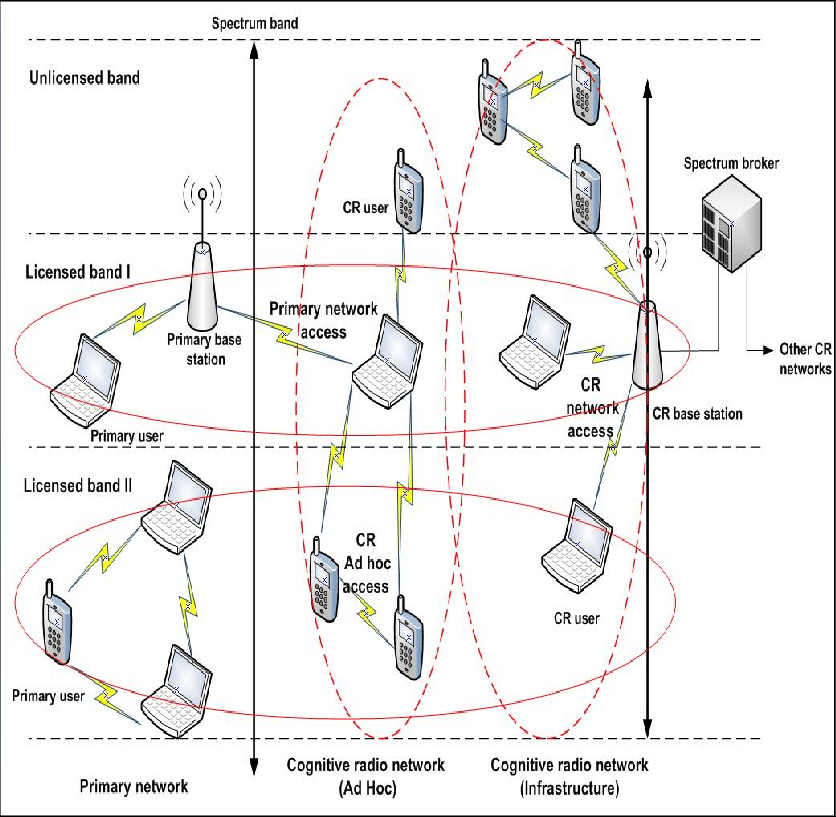
\includegraphics[width=0.6\textwidth]{myFigures/cogArch.png}
        \caption{Cognitive radio networks architecture~\cite{bwnGatechProjectDescription}}
        \label{fig:cogArch}
    \end{center}
\end{figure}

% Why is it interesting and important?
%The importance of our study lies on the fact that almost all the modern mobile devices contain multiple radios.

On the other hand, classical wireless networks frequently adopt the notion of deploying users with multiple radios~\cite{bahl2004reconsidering, adya2004multi}. An example multi-radio channel model is illustrated in Figure~\ref{fig:MIMO}. Such deployment of multiple radios improves capacity of the networks \cite{draves2004routing, bahl2004reconsidering}, enhances loss resilience \cite{miu2005improving}, and enables heterogeneous wireless access for smart devices \cite{song2012performance}. However, this augmentation also demands modified routing, medium-access, and link-layer protocols \cite{kyasanur2006routing, chatterjee2013low}. Nonetheless, as such deployment of multiple radios in wireless nodes is known to improve the performance of a user and  deployment of cognitive radios also aims to improve the performance of secondary users through spectrum utilization, it is intuitive that simultaneous utilization of both these techniques, i.e., Cognitive Multi-Radio Networks (CMRNs), will result in significantly improved network performance. Therefore, the notion of exploiting multiple radios in CRNs to supplement the dynamic spectrum access has been proposed in the contemporary literature. Existing studies in this regard present that such multi-radio deployment in CRNs improves delay up to a certain point, however, throughput always degrades with an increase in the number of radios per secondary user~\cite{khan2015towards}. Therefore, the main motivation behind this study is to examine how to improve network throughput while equipping secondary users with multiple radios.

\begin{figure}[!htbp]
    \begin{center}
        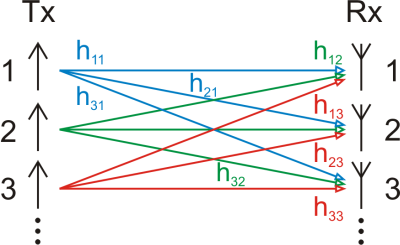
\includegraphics[width=0.55\textwidth]{myFigures/MIMO.png}
        \caption{Multi-radio channel Model~\cite{mimoWiki}}
        \label{fig:MIMO}
    \end{center}
\end{figure}

% Why is it hard? (E.g., why do naive approaches fail?)
The main challenge of improving total network throughput in CMRNs lies on the silent features of the architecture of CRNs. In CRNs, nodes generally have limited spectrum knowledge covering only its own neighborhood. Thus, the knowledge is conventionally gathered in a distributed manner. Therefore, graph-based and MILP optimization-based solutions~\cite{hoang2008downlink,ahmed2014channel} for improving throughput can not be directly incorporated due to their nature of performing centralized computations. Moreover, the relation between two different performance metrics (throughput and delay) may be opposing in nature~\cite{gamal2004throughput} and improving one of them may result in degradation of the another. Consequently, a trade-off between these two metrics demands special attention in CMRNs in road to improving throughput.

% Why hasn't it been solved before? (Or, what's wrong with previous proposed solutions? How does mine differ?)
Most of the existing studies on CMRNs fail to solve our research problem, as they overlook the effect of utilizing multiple radios on different performance metrics. The studies~\cite{de2012survey, feng2009joint, zhong2014capacity, li2014deterministic} usually integrate MAC and routing protocols for the multi-radio network architectures and solve the channel assignment problem for multi-channel scenario. While assigning multiple channels among multiple radios, the existing studies either randomly select the channels~\cite{khan2015towards} or only rank the channels~\cite{zhong2014capacity}. Due to all these reasons, to the best of our knowledge, no existing research study provides a viable solution for enhancing throughput in CMRNs.

% What are the key components of my approach and results? Also include any specific limitations.
To this end, in this paper, we propose to integrate feedback obtained from lower layers (Physical layer and Data Link layer) in the process of decision making in an upper layer (Application layer) to enhance network throughput. Here, to obtain lower layer feedback, we keep different packet counters for radios as well as channels in each secondary user. Using values of these counters, we rank all available radios and channels of a secondary user. Subsequently, based on the ranking, we make packet queuing decisions from the Application layer and channel switching decisions from the Data link layer while retaining a stochastic flavor. We implement our proposed feedback-based approach in \texttt{ns-3} to evaluate its performance in terms of throughput along with delay and drop ratio. Our simulation results demonstrate that the proposed approach can achieve significant improvement in terms of all the performance metrics in most of the cases.

% Summary of Contributions
%Then have a final paragraph or subsection: "Summary of Contributions". It should list the major contributions in bullet form, mentioning in which sections they can be found. This material doubles as an outline of the rest of the paper, saving space and eliminating redundancy.

%\section{Summary of Contributions}

Based on our study in this paper, we make the following set of contributions:

\begin{itemize}
\item We propose a feedback-based multi-radio exploitation approach, along with several variants, to solve the throughput degradation problem in CMRNs. In our proposed approach, performance information obtained from lower layers (Physical layer and Data link layer) is incorporated in the process of decision making of radio and channel selection.
\item We also evaluate the performance of our proposed approach through discrete-event simulation. We implement the proposed approach and its variants in \texttt{ns-3} to demonstate their radio selection and channel selection policies and measure various performance metrics in response to an increase in the number of radios per SU.
\item We compare performance of our proposed approach against that of existing approaches in the literature. Comparative results confirm significant improvement over existing approaches through using our proposed approach.
\item Our proposed approach increases total network throughput 51\% and decreases packet drop ratio up to 35\% on an average against that of existing approaches.
\item At last, we also provide several research questions in the domain of CMRNs to guide future research direction.
\end{itemize}
\endinput
